The design of the software, architecture, and technologies used to create the web-application and databases are described in the following section. The analysis being performed by the web-application, how it performs each analysis, and how the back-end queries each database is discussed.

\subsection{Database Technologies}

This section covers the underlying technologies used to implement the databases being benchmarked. This is important to note in terms of how portable each technology is, how difficult the configuration is before each database can be used for a given project, or limitations on performance or hardware requirements due to software requirements. While each database technology has varying capabilities, in terms of being supported for a given operating system, they each provide support for being deployed in a containerized environment.

\edt{It is important to note that JanusGraph and TigerGraph differ in an important way regarding each database's implementation of their graph schema rules. TigerGraph advertise their product as an analytics platform so these kinds of design decisions may fall back on this point. JanusGraph is schemaless, so new keys can be defined at anytime, whereas TigerGraph's schema must be defined beforehand, very much as in the case of relational databases. TigerGraph has vertex-attached accumulators if values attached to vertices during a query is important, but if this information is to be persisted it needs to be a part of the schema.}

\subsubsection{PostgreSQL}
PostgreSQL is written in the C programming language, is an object-oriented relational database, and is queried via SQL commands. PostgreSQL, like many relational databases, is ACID-compliant and robust to transactional failures. It is built to be extensible with a variety of extensions one can install for additional features such as UUID or spatial indexing. PostgreSQL can be deployed on a variety of major operating systems such as Windows, Mac, Linux (Redhat, Debian, and a few others), Solaris, and BSD.

PostgreSQL is a mature product and has a large amount of support from its open-source community. Postgres is flexible in that it supports a variety of data types and allows the definition of own types. Founder of NewsBlur\footnote{\url{https://newsblur.com/}}, Samuel Clay, mentions using Postgres for multiple years for storing millions of sites and subscriptions. Canonical\footnote{\url{https://canonical.com/}} founder, Mark Shuttleworth, explains that, while using Postgres during the development of Launchpad, finding it ``robust, fast, and professional in every regard'' \cite{postgresAbout}.

Many of these features and opinions of using PostgreSQL in production environments on this scale is why PostgreSQL was a reputable relational database to benchmark against. PostgreSQL 11 and PostGIS 2.5 are used in this investigation.

\subsubsection{JanusGraph}

JanusGraph is a highly scalable graph database that is ready to be clustered between multiple machines. It is a transactional database which supports ACID-compliance and eventual consistency \cite{janusgraphMain}. It is written in Java and is thus platform independent. JanusGraph is a project under The Linux Foundation and is forked from the Titan project as a continuation of the vision in creating an open-source, scalable, highly concurrent graph database. There is support for those wishing to migrate from Titan in order to benefit from the bug fixes and additional features now supported via JanusGraph \cite{janusgraphTitan}.

JanusGraph is largely based on the Apache tech-stack making use of technologies such as Apache TinkerPop\footnote{Thus makes use of the property graph model.}, Lucene, Cassandra, Hadoop, and more. This adds to complexity when configuring JanusGraph as, for each technology plugged in, there may be configuration necessary. Gremlin is the native language through which JanusGraph is queried but, as mentioned in Section \ref{subsec:lang}, can be extended for Cypher queries. JanusGraph benefits from optional support for advanced search capabilities and having no-single point of failure \cite{janusgraphDocs}.

\begin{figure*}[h]
    \centering
    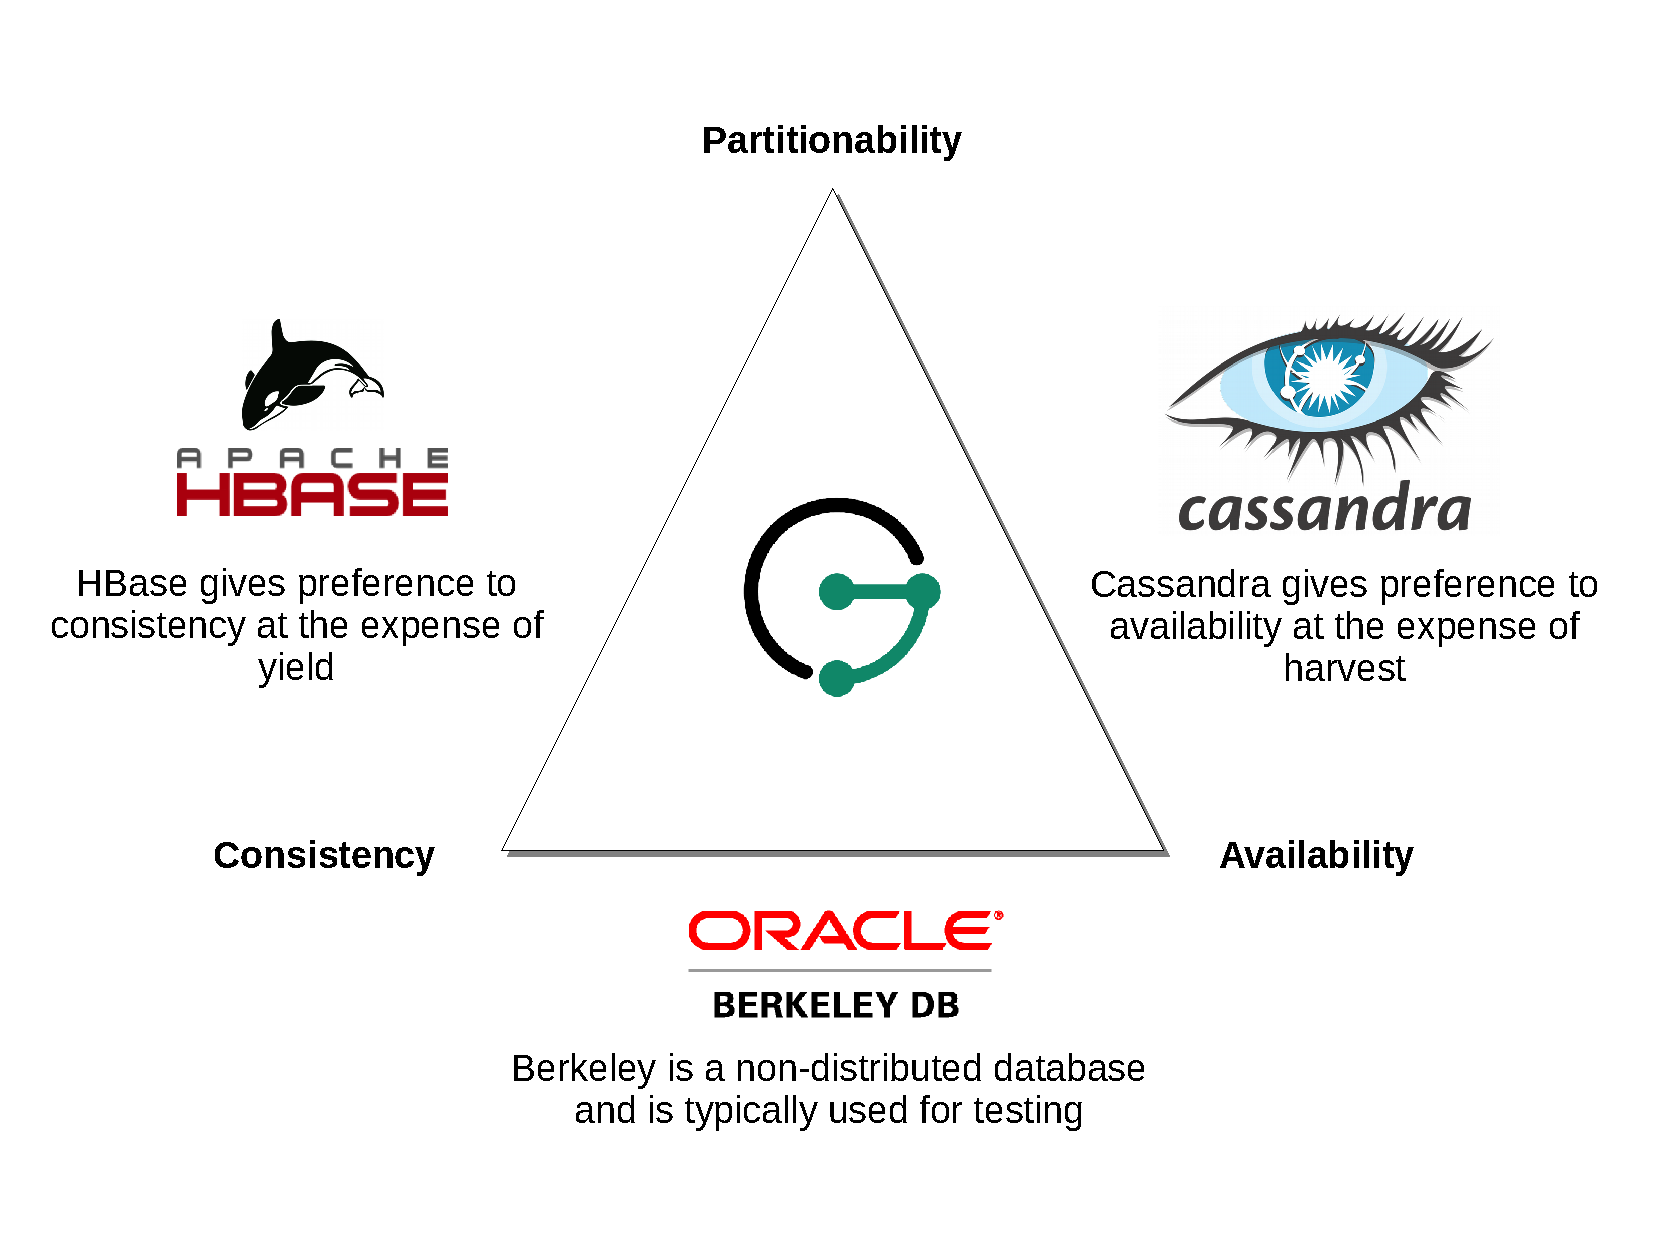
\includegraphics[width=10cm]{img/5_designFigures/cap.pdf}
    \caption{The CAP theorem illustrated using JanusGraph's three supporting storage back-ends. This diagram is largely inspired from Chapter 1 in Titan's documentation and is adjusted for JanusGraph \cite{titanCap}.}
    \label{fig:janusgraphCap}
\end{figure*}

JanusGraph can store graph data via three supporting back-ends; Apache Cassandra, Apache HBase, and Apache Berkeley. The CAP Theorem (Section \ref{cap}) should be taken into account when considering which of the three back-ends to use -- this is illustrated in Figure \ref{fig:janusgraphCap}.

Examples of companies who have deployed JanusGraph in production include Netflix, Redhat, Uber, and IBM \cite{janusgraphReadme}. The professional support, documentation, and fact that one is able to leverage all these advanced features for free is why JanusGraph is one of the graph databases used in this investigation. The configuration of JanusGraph used in this paper is with Apache Cassandra as the storage back-end and ElasticSearch as the search engine for spatial and temporal query support. JanusGraph 0.4 is used in this investigation.

\subsubsection{TigerGraph}

TigerGraph is an enterprise level graph analytics platform developed in the C++ programming language. TigerGraph was developed with hindsight from projects such as Apache TinkerPop and Neo4j and provides features such as native parallel graph processing and fast offline batch loading \cite{tigergraphBenchmark} \cite{conferenceTrip}. Unlike JanusGraph, TigerGraph was developed from scratch in order to effectively create the next generation of graph database technology. TigerGraph won Strata Data’s ``Most Disruptive Startup'' Award for its return in this decision \cite{tigergraphAward}.

Some of the use cases explicitly mentioned by TigerGraph\footnote{\url{https://www.tigergraph.com/solutions/}} are in geospatial and time series analysis. This lends itself as a promising database technology for this investigation. TigerGraph is queried using their GSQL querying language (see Section \ref{subsec:lang}) where queries are optimized via an installation process where a REST endpoint is also generated in the process. Like JanusGraph, TigerGraph can be deployed on multi-machine clusters, but this is limited to the enterprise version of this product. TigerGraph uses Apache Zookeeper for cluster management and Apache Kafka for message queuing.

GraphStudio is a web interface which is packaged along with TigerGraph which provides an interface to write, install and visualize queries, design and export one's graph schema, and monitor database performance. This makes use of an Nginx web server \cite{tigergraphInfoworld}.

For all intents and purposes, the developer edition is more than capable to perform the investigation required for this paper. There is an enterprise version that allows for additional features such as multi-machine clustering. TigerGraph 2.5 is used in this investigation.

\subsection{Web-application Simulation}

The web-application, called Providentia\footnote{The name of the web-application is a nod to JanusGraph and Titan's theme of Roman mythology. Providentia is associated with provision and forethought \cite{providentiaMeaning}. This was thought to be fitting due to the nature of our experiments designed to find the best database for storing and modeling our particular data.}, is used to queue analysis in a pipeline on which each benchmark is to be run, server performance measured, and accumulated results be displayed. This is deployed on target hardware and will import a subset of the data determined by a configurable percentage. Then one will be able to use the web-based interface to perform all necessary benchmarking tasks.

The architecture and how each technology communicates is illustrated in Figure \ref{fig:providentiaArchitecture}. The databases are containerized using Docker\footnote{\url{https://www.docker.com/}}.

\begin{figure}[h]
    \centering
    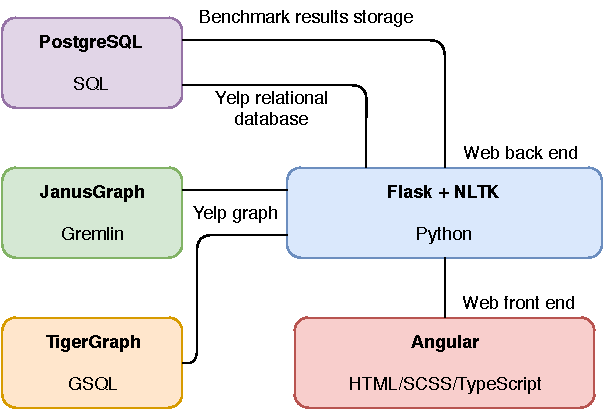
\includegraphics[width=0.49\textwidth]{img/5_designFigures/providentiaArchitecture.pdf}
    \caption{The architecture of Providentia.}
    \label{fig:providentiaArchitecture}
\end{figure}

JanusGraph has some Java specific features that add limitations when making use of embedded Gremlin in Python. The limitations are, when trying to make use of mixed indexing search predicates such as spatial queries, that one may only do this via Java or a superset language thereof. The workaround for this was to make use of the Gremlin Translator which takes a Gremlin query as a string and interprets it on the server side.

The first motivation towards using a Python back-end is that the text in the reviews can be analysed using NLTK for easily implemented sentiment analysis. The second is that a simple REST API can be easily and quickly designed and deployed using the Flask framework. Angular was subjectively chosen as the front end framework as it allows for fast front end web development. All benchmarking results are stored in a separate database within PostgreSQL.

The front end of Providentia allows a user to query each database, test the sentiment classifier, add benchmarking jobs and to review the performance and results of each analysis. Each job is run serially to avoid too much interference and competition between each database for resources. At intervals the CPU performance and memory consumption is measured and stored in PostgreSQL. The server performance and results of an analysis can be viewed together to validate that the outputs are the same and how each database utilizes the server's resources.

\subsection{Data Analysis}
Using each of the databases, a number of data analysis jobs are performed on the data. This section describes what each analysis aims to do and how they align to a typical real world use case. Each of these jobs have some kind of spatiotemporal aspect to test the accessibility of the data to demonstrate how well the given database handles the data.

These analysis are run over different percentages of the data loaded in each database and the performance is then measured and discussed in Section \ref{sec:experiments}. This section goes into more detail about the types of queries written and how well each language expresses each
query.

\subsubsection{Sentiment Analysis}
One application for graph analytic platforms is in machine learning. In order to further build context around each of the kernels mentioned in the next section, a simple binary sentiment classifier is used to classify the text of reviews as representing either a positive or negative sentiment. Sentiment analysis is a class of natural language processing where subjective information is extracted from a given text \cite{sentimentAnalysisGupta}.

Although this investigation does not explore the applications of machine learning models on spatiotemporal data, it will explore how it could reveal interesting information alongside patterns among the data. All natural language processing is done using the Natural Language Toolkit (NLTK)
\footnote{\url{https://www.nltk.org/}} for Python.

\subsubsubsection{Machine Learning Model}
NLTK's Na\"ive Bayes classifier\footnote{\texttt{nltk.NaiveBayesClassifier}} was used as the model to train and classify sentiment. Na\"ive Bayes is a probabilistic machine learning model which has proven very effective in text classification. A limitation of this model, on a binary classification problem, includes only being able to perform linear separability. This should not be an issue regarding the use of adjectives as feature vectors, since the most informative adjectives seem to be verbose and particular to a specific sentiment e.g. words such as horrible, disgusting, perfect, and wonderful \cite{rish2001empirical}.

One problem faced by sentiment analysis is that of negation which may make certain adjectives less information e.g. good vs not good \cite{blanco2011some}. Nevertheless, the model performs well in terms of separating the two classes.

\subsubsection{Kernels}
\label{sec:kernels}

Each of the following kernels represent some kind of user story for data analysis. Each one has some spatio-temporal constraint which will be applied on the respective queries. Each of these kernels will be benchmarked 30 times each such that the mean and standard deviation can be considered when comparing response times. 

For each kernel, their respective database queries are available in Appendix \ref{app:queries}.

\subsubsubsection{Medical: Priority 1 Mean Response Times}

\edt{This analysis looks at the mean of two intervals within the response life cycle namely; travel time to the hospital and the time taken for the ambulance to start driving to the patient. This will filter out all responses which do not take the patient to the hospital and responses without a priority of 1 (highest).}

\edt{One hospital is isolated during this query. This query is useful in post-simulation analysis when optimizing response times with respect to a specific hospital. This can be extended to be grouped by hospitals if labels are associated with the coordinates.}

\subsubsubsection{Medical: Second Resource to Transfer Patients}

\edt{During a response, sometimes multiple resources need to be sent depending on varying evaluation criteria made either by the call receiver or first resource upon arrival at the scene. This analysis considers how many resources, grouped by priority, were sent as the second resource to the same destination hospital from the kernel used above. This analysis can be used to investigate each priority's resource usage and if their priority was perhaps misclassified. It can be further extended to look at third and fourth resources in order to be more thorough with the analysis.}

\subsubsubsection{Medical: Long Response Count}

\edt{This analysis is purely temporal and combines the time intervals from when the ambulance leaves up until the point where the patient is delivered to a hospital. The number of responses are returned for all responses which take longer than 15 minutes. This analysis could be useful when considering introducing a new hospital into a given area to improve response times.}

\subsubsubsection{Yelp: Kate's Restaurant Recommendation}

This analysis selects a user near the beginning of the dataset named Kate. This user has a number of reviews for restaurants in the Las Vegas area. A subset of reviews which hold a strictly greater than 3 star rating by Kate are selected, sorted by date descending, and limited by 10 reviews per user in order to take the most relevant ones. These businesses are then selected, filtered by category ``Restaurants''. The users who have a star rating equal to or greater than Kate's ratings for the same businesses are selected as the recommending users.

Now assume that Kate has relocated to a new area. All businesses which have been rated strictly larger than 3 stars by the recommending users are then selected as restaurants to recommend to Kate in the new area. The text in these reviews are checked for sentiment and the percentage positive sentiment is displayed alongside the average star rating for each recommended restaurant. This sentiment vs. average star rating is used as a metric to analyse in terms of asking the question: How reliable is the star rating versus the actual sentiment found in the text?

The purpose of the first part of this kernel is to test the performance of a 1-hop graph traversal pattern. This hop is demonstrated in category filtering and finding users with mutual sentiment for a given review. This type of situation is faced by many recommendation technologies and this is quite a basic technique for recommendation. The additional challenge is the relocation of Kate and seeing how responsive the database is to the spatial and temporal aspect which is the second part of this kernel. The accumulated list of users is split into a separate query for each user to test the ability of each database technology to perform concurrent reads on subsets of data which is a strength of NoSQL databases.

\subsubsubsection{Yelp: Review Trends in Phoenix 2018}

This analysis goes deeper into observing the trend of various characteristics of reviews versus their star ratings. This is a common analysis performed on the Yelp dataset \cite{yelpTrendsZhang}, but the version in this investigation selects a subset of reviews only within the 2018 year in the Phoenix area. The spatiotemporal boundaries placed on this subset may reveal hidden trends to be considered in future work.

Reviews are extracted first by location (which results in a much smaller subset than extracting by date first) then by date. The reviews are then separated by star rating. For each star rating, the characteristics of ``funny'', ``useful'', and ``cool'' are accumulated and the text is classified as either positive or negative. For each star rating these are normalized and placed next to one another to see the characteristic of a review from each star group. Below is a comparison of the queries written for this kernel.

\paragraph{SQL}

This kernel is the least complex of the three as it has a single join with a spatio-temporal constraint. Listing \ref{lst:sqlReviews2018} returns selected characteristics on reviews where the date year is 2018 and reviewed businesses are within the Phoenix area.

\lstinputlisting[
    language=sql,
    caption={
        A SQL query that returns all the review text and ratings for businesses within 50km of the Phoenix area during 2018.
    },
    label={lst:sqlReviews2018}
]
{./queries/yelp2/reviews.sql}

\paragraph{Gremlin}

One caveat of using mixed indexes on dates via the Gremlin Translator is highlighted in the query for this kernel. Usually, since Gremlin is designed to be embedded, one should make use of objects when appropriate. Since JanusGraph is being queried from Python\footnote{Where ideally, it would be within a JVM language which has access to the JanusGraph specific classes and functions, e.g. Groovy.}, with no support for mixed query specific parameters, date related parameters need to be parsed using static methods from the \texttt{Instant} class in Java. This can be seen in Listing \ref{lst:gremlinReviews2018} when filtering reviews by date. Alternatively, one could also use the \texttt{filter} step as is done in Listing \ref{lst:gremlinCityAppen}.

Out of the set of businesses within the Phoenix area and set of all the reviews in 2018, the businesses set would be the smaller of the two. This is important when using a dataflow language since the whole subset will be accumulated before moving to successive functions in the query. Due to this characteristic of Gremlin, businesses are accumulated before the reviews.

\lstinputlisting[
    language=gremlin,
    caption={
        A Gremlin query that returns all the review text and ratings for businesses within 50km of the Phoenix area during 2018.
    },
    label={lst:gremlinReviews2018}
]
{./queries/yelp2/reviews.groovy}

\paragraph{GSQL}

Since only selected characteristics of a review are desired, a tuple is created at the beginning of Listing \ref{lst:gsqlReviews2018}. The businesses within the Phoenix area are selected first, then reviews where the date part is 2018. The review tuples are accumulated into a \texttt{ListAccum}.

\lstinputlisting[
    language=gsql,
    caption={
        A GSQL query that returns all the review text and ratings for businesses within 50km of the Phoenix area during 2018.
    },
    label={lst:gsqlReviews2018}
]
{./queries/yelp2/reviews.gsql}

\subsubsubsection{Yelp: Ranking Las Vegas by Friends' Sentiment}

The purpose of this analysis is the ability to aggregate relations from depth 1 -- 2 of a graph pattern while maintaining spatio-temporal constraints. The user story of this kernel is that a user in the dataset would like to travel to Las Vegas over the Nov -- Dec period. Instead of asking from each of the hundreds of direct friends to thousands of mutual friends, the sentiment from their reviews written during the Nov -- Dec period (irrespective of year) in the Las Vegas area will be analysed.

Both friends and mutual friends will be aggregated and all reviews written during the Nov -- Dec period will be filtered. These reviews will be filtered by the spatial constraint of whether they are connected to businesses within 30km of the Las Vegas center. The remaining reviews will have their text data extracted and returned for analysis. Using the sentiment classifier, a percentage positive sentiment will be generated and this will be the result of the data analysis.
